\documentclass{article}
\usepackage{scrextend}
\usepackage[utf8]{vietnam}
\usepackage{titling} 
\usepackage{setspace}
\usepackage[a4paper, total={170mm,257mm},left=25mm,right=25mm, top=20mm]{geometry}
\usepackage{unicode-math}
\usepackage{amsfonts}
\usepackage{amsmath}
\DeclareMathOperator*{\argmax}{arg\,max}
\usepackage[symbol]{footmisc}
\makeatletter
\newcommand\footnoteref[1]{\protected@xdef\@thefnmark{\ref{#1}}\@footnotemark}
\makeatother
\usepackage{footnotehyper}
\usepackage{perpage} %the perpage package
\MakePerPage{footnote}

\usepackage{scrextend}
\usepackage{scrextend}
\title{\textbf{Phát hiện COVID-19 và viêm phổi \\ bằng ảnh X-quang sử dụng mạng neural tích chập\footnote[1]{Đây là báo cáo đồ án môn học Nhập môn Thị giác máy tính - CS231.L23.KHCL tại trường Đại học Công nghệ Thông tin - ĐHQG HCM}}}
\setlength{\parindent}{0pt}
\usepackage{indentfirst}
\setlength{\parindent}{0pt}
\usepackage{ragged2e}
\usepackage[english]{babel}
\usepackage[square,numbers]{natbib}
\usepackage[colorlinks, citecolor = black, urlcolor = gray, bookmarks = false, hypertexnames = true ]{hyperref} 
\bibliographystyle{abbrvnat}
\author{
  \textbf{Phạm Ngọc Tân}\\
  \small 19520925@gm.uit.edu.vn
  \and
  \textbf{Võ Khánh An}\\
  \small 19520007@gm.uit.edu.vn}
 
\date{Tháng 07/2021}

\usepackage{graphicx}

\usepackage[ruled, lined, linesnumbered, commentsnumbered, longend]{algorithm2e}
\usepackage{xcolor}
\usepackage{mathtools}
\usepackage[]{algorithm2e}

\begin{document}

\maketitle

\begin{abstract}
\justifying 
\noindent 
    Hiện nay, tình hình COVID-19 của Việt Nam và cả thế giới đang trở nên vô cùng phức tạp. Đó là lý do tại sao chúng ta cần phải có hành động kịp thời để có thể ứng phó với cơn đại dịch này và bước đầu trong công cuộc ứng phó này phải kể đến việc xác định đâu là các nhiễm COVID-19. Vì thế nên trong bài báo cáo này, chúng tôi sẽ giới thiệu một phương pháp xét nghiệm COVID có độ hiệu quả cao trong thời gian ngắn, sau đó sẽ áp dụng phương pháp đó lên nhiều mô hình máy học khác nhau và tiến hành phân tích ưu nhược điểm của các mô hình này để có một cái nhìn tổng quan hơn về việc áp dụng trí tuệ nhân tạo vào xét nghiệm nhanh COVID-19.
\end{abstract}

% /--------------------------------/
\section{Giới thiệu}
\subsection{Về số liệu thống kê}
Tình hình dịch COVID-19 hiện nay là một vấn đề cấp bách không chỉ với Việt Nam, mà còn ở toàn thế giới. Cụ thể, tính đến $18h$ ngày $16/6/2021$ theo giờ Việt Nam, toàn thế giới ghi nhận hơn $177.470.620$ ca nhiễm COVID-19, trong đó, $3.839.931$ ca tử vong và $161.919.653$ ca đã bình phục. Ngoài ra, trong vòng $24h$ từ ngày $15/6$ đến $16/6/2021$, cả thế giới ghi nhận hơn $313.790$ ca mắc COVID-19 và $9.749$ ca tử vong \cite{worldometers}.\\

Còn ở Việt Nam, dữ liệu được cập nhật đến $18$h ngày $21/5/2021$, tổng cộng có $4.941$ người nhiễm COVID-19, trong đó có $2.689$ ca khỏi bệnh và $41$ ca tử vong. Và trong vòng ngày $19/6/2021$, có thêm $470$ ca nhiễm mới \cite{ncov}.\\

\subsection{Về phương pháp xét nghiệm}
Để đối phó với dịch bệnh viêm đường hô hấp cấp này, các y bác sĩ đã có khá nhiều những phương pháp để có thể chẩn đoán nhanh những ca mắc virus SARS-CoV-2. Tuy nhiên, phương pháp được cho là có hiệu quả và phổ biến hơn cả chính là phương pháp xét nghiệm nhanh COVID bằng phản ứng chuỗi Polymerase.
\subsubsection{Xét nghiệm sinh học phản ứng chuỗi Polymerase thời gian thực}
\textit{Phản ứng chuỗi Polymerase} (PCR) là một phản ứng nhân bản DNA dựa trên các chu kì nhiệt. Và \textit{xét nghiệm sinh học phân tử chuỗi Polymerase} (RT PCR) là phương pháp xét nghiệm xác định sự hiện diện của virus thông qua phát hiện vật liệu di truyền của virus SARS-CoV-2 \cite{ncov}. Đây là một phương pháp có độ chính xác cao nhưng lại đòi hỏi các hệ thống máy chuyên dụng và cần phải được thực hiện tại các phòng thí nghiệm.\\

Ưu điểm của RT PCR đó chính là nó có độ uy tín và độ chính xác cao. Tuy nhiên nhược điểm lại chính là việc nó thường chỉ được sử dụng cho những ca nghi nhiễm virus SARS-CoV-2, không thể áp dụng rộng rãi với toàn dân vì đây là phương pháp tốn khá nhiều nhân công (thường là những người có trình độ cao về y học) và phải ở trong môi trường đặc thù như phòng thí nghiệm, cho nên phương pháp này có giá thành khá cao: $734.000$ VNĐ cho 1 lần xét nghiệm \textit{(theo thông tư 5834 của Bộ Y tế)}. Phương pháp này cũng không có tính ổn định tuyệt đối vì vẫn có trường hợp 2 - 3 lần đầu là âm tính nhưng lần tiếp theo là dương tính. Ngoài ra, cũng xuất hiện các trường hợp dương tính giả và âm tính giả khi xét nghiệm nhanh Covid bằng RT PCR (tại vì số lượng virus nhân lên chưa đủ lớn và xuất hiện nhiều trong đường hô hấp, hoặc do kĩ thuật lấy mẫu và điều kiện lấy mẫu chưa chuẩn, hoặc thậm chí là do quá trình vận chuyển và bảo quản mẫu xét nghiệm chưa đúng cách).

\subsubsection{Chẩn đoán hình ảnh}
Ngoài RT PCR, còn có một phương pháp khác giúp bác sĩ có thể xác định nhanh những ca COVID. Đó chính là phương pháp chẩn đoán hình ảnh bằng ảnh X-quang.\\

Phương pháp chẩn đoán hình ảnh này là một phương pháp nhanh hơn rất nhiều so với xét nghiệm nhanh Covid bằng RT PCR. Ngoài ra, giá thành của chẩn đoán hình ảnh bằng ảnh X-quang là thấp, chỉ vào khoảng $100.000$ VNĐ trên 1 người trên 1 lần chụp.\\

Tuy nhiên, nhược điểm của phương pháp này chính là việc các bác sĩ khó có thể chẩn đoán chính xác hoàn toàn các ca nhiễm COVID chỉ sử dụng ảnh X-quang, mà các bác sĩ còn phải cần dùng những đặc điểm dịch tễ và những biểu hiện lâm sàng khác để có thể đưa ra các chẩn đoán phù hợp. Điều này vô hình chung lại gây nên sự thiếu hụt về nguồn nhân lực về y tế vì phương pháp này chỉ có thể sử dụng bởi những y bác sĩ hàng đầu về chẩn đoán hình ảnh. Một nhược điểm khác trong chẩn đoán hình ảnh đó chính là tình trạng nhầm lẫn giữa COVID-19 và bệnh viêm phổi.\\

\subsubsection{Chẩn đoán hình ảnh sử dụng trí tuệ nhân tạo}
Để cải thiện những hạn chế mà phương pháp chẩn đoán hình ảnh truyền thống tạo ra, chúng tôi giới thiệu một phương pháp chẩn đoán mới có thể giúp cho các y bác sĩ giảm thiểu được không chỉ về chi phí cần bỏ ra cho những lần xét nghiệm, mà còn giúp giảm thiểu những hạn chế về nhân lực như đã nêu ở phần trên.\\

Vì chẩn đoán hình ảnh bằng ảnh X-quang có một chi phí tương đối thấp, cho nên ta có thể áp dụng việc chẩn đoán này để có thể xét nghiệm Covid diện rộng mà không bị trở ngại về chi phí. Ngoài ra, áp dụng trí tuệ nhân tạo (AI) để chẩn đoán cũng giúp tăng đáng kể tốc độ chẩn đoán COVID khi AI cho ra kết quả ngay lập tức thay vì ta phải chờ 2 3 tiếng như RT PCR. Chúng ta có thể sử dụng việc chẩn đoán hình ảnh diện rộng để bước đầu xác định được những ca dương tính, sau đó chúng ta sẽ tiến hành làm xét nghiệm nhanh Covid bằng RT PCR để có thể kiểm tra lại. \\

Ngoài ra đối với những người đã phơi nhiễm hoặc bị nhiễm COVID-19 thì trong thời gian cách ly và chữa trị, chúng ta có thể áp dụng chẩn đoán hình ảnh đến khi nào người đó có kết quả chẩn đoán là âm tính thì ta có thể kiểm tra lại bằng RT PCR. Điều này giúp chúng ta có thể tiết kiệm ngân sách một cách rõ rệt (cụ thể, giảm chi phí đi gấp 7 lần so với việc sử dụng RT PCR mỗi lần cần kiểm tra). \\

Và vì AI không cần đến nguồn nhân lực dồi dào và đặc thù để có thể sử dụng nên ta có thể tiết kiệm được nguồn nhân lực, nhất là nguồn nhân lực của y bác sĩ.

% /--------------------------------/
\section{Cơ sở luận cho chẩn đoán COVID-19 bằng ảnh X-quang}
Để có thể áp dụng AI cho việc chẩn đoán COVID-19, cũng như phân biệt giữa COVID-19 và viêm phổi, chúng ta cần phải biết được một số đặc điểm nhất định của cả 2 nền bệnh khi chỉ nhìn vô ảnh chụp X-quang. Như chúng ta có thể thấy ở ảnh dưới đây:
\newpage
\begin{figure}[h!]
  \centering
    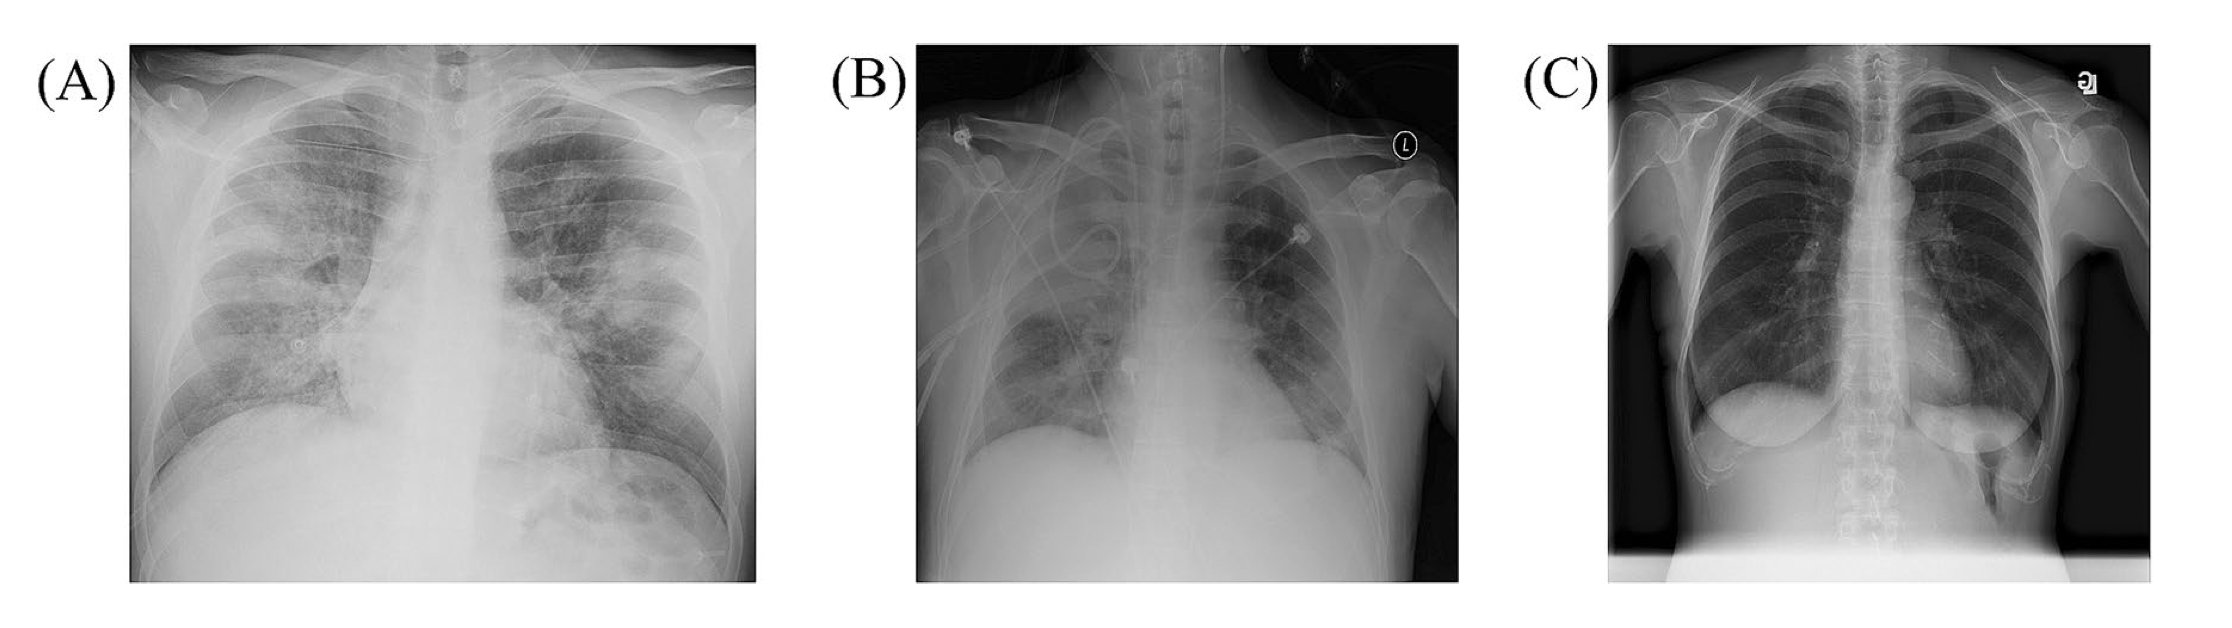
\includegraphics[width=\textwidth]{covid+pneumonia+normal.png}
\end{figure}
\begin{center}
    Hình 1. Ảnh X-quang cho các trường hợp:\\ Bệnh nhân COVID-19 (A), bệnh nhân viêm phổi (B) và người không bị bệnh về đường hô hấp (C)
\end{center}

Ảnh X-quang phổi của bệnh nhân viêm phổi và bệnh nhân COVID khác với phổi bình thường đó chính là việc phổi của những người mắc bệnh có xuất hiện các đốm trắng nhiều hoặc ít ở những vị trí khác nhau trong phổi. \\

Những đốm trắng này trong y khoa được gọi là \textit{hình ảnh kính mờ} (ground glass pattern). Hình ảnh kính mờ là tổn thương đông đặc không hoàn toàn, có tỷ trọng cao hơn nhu mô phổi xung quanh vẫn có thể thấy đường bờ các mạch máu hoặc phế quản bên trong tổn thương đó.\\

Một bác sĩ chuyên gia về chẩn đoán hình ảnh có thể nói rằng những hình ảnh kính mờ này chính là nguyên nhân gây nên những đốm trắng trong ảnh. Và các bác sĩ có thể dùng đặc trưng này để phân biệt bệnh nhân COVID hay viêm phổi. Vì thế cho nên có thể biết được rằng khi sử dụng những mạng học sâu, các mô hình máy học sẽ học dựa trên những đặc điểm hình thái này và cho ra kết quả chẩn đoán phù hợp nhất với từng ca bệnh. 

% /--------------------------------/
\section{Các phương pháp}
Trong đồ án này chúng tôi tận dụng sức mạnh của hai mạng neural là VGG19 \cite{vgg19} và ResNet50 \cite{resnet50}. Cả hai kiến trúc mạng này đã chứng minh được hiệu quả của mình qua các ứng dụng trong thực tế. Bên cạnh đó chúng tôi cũng sử dụng COVIDx dataset, một bộ dữ liệu được sử dụng rất nhiều trong các nghiên cứu về COVID-19 hiện nay.

\subsection{COVIDx Dataset}
COVIDx Dataset \cite{covidxdataset} là một bộ dữ liệu được tổng hợp từ nhiều tập dữ liệu khác nhau, cụ thể: \citet{data1}, \citet{data2}, \citet{data3}, \citet{data4}, và \citet{data5}. Ngoài ra, bộ dữ liệu này cũng cung cấp một công cụ chuyển ảnh y khoa từ định dạng .mri thành định dạng .jpg. Thêm vào đó, tác giả cũng cung cấp một đoạn mã giúp hỗ trợ tiền xử lý, lược bỏ những thành phần không cần thiết cho bộ dữ liệu đã được tổng hợp.\\

Bộ dữ liệu gồm hơn $20.000$ ảnh X-quang phổi từ những bệnh nhân khác nhau, được chia làm 2 tập: tập train và tập test, và được phân thành 3 lớp lần lượt là: viêm phổi (train: 5963, test: 105), COVID-19 (train: 4649, test: 274) và bình thường (train: 8751, test: 100).\\

Mô hình sẽ lấy vào input là một ảnh chụp X-quang phổi và sẽ cho ra ouput là xác suất ảnh chụp X-quang đó rơi vào từng lớp viêm phổi, COVID-19 và bình thường.

\subsection{Chi tiết thực hiện}
Cả hai mạng học sâu là VGG19 và ResNet50 chúng tôi đề xuất đều đã được pretrained trên ImageNet \cite{imagenet}. Sau đó chúng tôi tiến huấn luyện trên tập dữ liệu COVIDx với thuật toán tối ưu hóa là Adam và chiến lược là learning rate sẽ giảm khi nếu loss của tập validation không cải thiện sau một khoảng thời gian (patience).\\

Đối với mạng VGG19, các siêu tham số chúng tôi sử dụng cho huấn luyện là: learning rate = 5e-4, số lượng epoch = 13, kích thước batch = 32, factor = 0.1, patience = 3 và độ phân giải của ảnh đầu vào = 480x480.\\

Trong khi đó đối với mạng ResNet50, chúng tôi thực hiện huấn luyện 2 lần riêng biệt, cụ thể:
\begin{itemize}
    \item Các siêu tham số cho lần đầu tiên là: learning rate = 5e-4, số lượng epoch = 14, kích thước batch = 32, factor = 0.1, patience = 3, độ phân giải của ảnh đầu vào = 224x224.
    \item Các siêu tham số cho lần thứ hai là: learning rate = 5e-3, số lượng epoch = 50, kích thước batch = 32, factor = 0.1, patience = 3, độ phân giải của ảnh đầu vào = 224x224.
\end{itemize}

Ngoài ra, chúng tôi cũng cắt giảm một số hình ảnh trong lớp viêm phổi và bình thường để đảm bảo sự cân bằng về số lượng hình ảnh trong cả 3 lớp của bài toán. Đồ án này chúng tôi đã xây dựng và đánh giá chủ yếu trên tư viện học sâu Keras và framework Tensorflow.

% /--------------------------------/
\section{Kết quả thực nghiệm và đánh giá}
Để tiến hành kiểm tra chất lượng của các mô hình, chúng tôi đã sử các phương pháp đánh giá như độ chính xác, possitive predictive value (PPV), sensitivity và F1-score. Như trong bảng 1, độ chính xác mô hình VGG-19 của chúng tôi đạt 86\%, kết quả này tốt hơn 3\% so với \cite{covidxdataset}. Tuy nhiên, ResNet50 của chúng tôi thể hiện rất kém, điều này có thể lý giải vì độ phân giải ảnh đầu vào của chúng tôi chỉ là 224x224 (do hạn chế phần cứng), thay vì 480x480. 
\begin{center}
        \begin{tabular}{|c|c| c|c| c|c| c|c| c|c|}
        \hline
            Kiến trúc & Số lượng tham số (triệu) & Độ chính xác & Độ phân giải ảnh đầu vào\\
            \hline
            VGG19 \cite{covidxdataset} & 20.37 & 83$\%$ & \\
            \hline
            VGG19 & 29.76 trainable + 20.25 non-trainable & 86$\%$ & 480 x 480\\
            \hline
            ResNet50 \cite{covidxdataset} & 24.97 & 90.6$\%$ & \\
            \hline
            ResNet50 (14 epochs) & 25.93 trainable + 23.77 non-trainable & 77$\%$ & 224 x 224\\
            \hline
            ResNet50 (50 epochs) & 25.93 trainable + 23.77 non-trainable & 84$\%$ & 224 x 224 \\
            \hline
            COVID-net \cite{covidxdataset} & 11.75 & 93.3$\%$ & 480 x 480\\
        \hline 
        \end{tabular}
    \end{center}
\begin{center}
    Bảng 1. So sánh độ chính xác và lượng tham số giữa các mô hình 
\end{center}
Tiếp theo, chúng tôi tiến hành so sánh dựa trên thống số sensitivity. Mạng VGG19 của chúng tôi thể hiện vượt trội so với mạng VGG của \cite{covidxdataset} trên độ đo này. Ngoài ra các con số khác trong bảng này trên mạng ResNet50 (epoch) và VGG19 của chúng tôi đều đạt kết quả hết sức khả qua, tất cả đều từ 80$\%$ trở lên. Việc đạt được các kết quả sentivity cao là rất quan trọng bởi điều này nói lên rằng các mô hình bỏ sót rất ít các bệnh nhân trên các lớp. Đây là việc hết sức cần thiết bởi chúng ta không hề muốn một mô hình tuy dự đoán chính xác nhưng lại bỏ sót các trường hợp nhiễm COVID-19 trong bối cảnh dịch bệnh như hiện nay.
\begin{center}
        \begin{tabular}{|c|c| c|c| c|c| c|c| c|c|}
        \hline
            Kiến trúc & Không mắc bệnh về đường hô hấp & Viêm phổi & COVID-19\\
            \hline
            VGG19 (\citeauthor{covidxdataset},\citeyear{covidxdataset}) & 98\% & 90\% & 58.7\% \\
            \hline
            VGG19 & 96\% & 86\% & 82\%\\
            \hline
            ResNet50 (\citeauthor{covidxdataset},\citeyear{covidxdataset}) & 97\% & 92\% & 83\% \\
            \hline
            ResNet50 (14 epochs) & 96\% & 85\% & 67\%\\
            \hline
            ResNet50 (50 epochs) & 86\% & 90\% & 80\%\\
            \hline
            COVID-net (\citeauthor{covidxdataset},\citeyear{covidxdataset}) & 95\% & 94\% & 91\%\\
        \hline 
        \end{tabular}
    \end{center}
\begin{center}
    Bảng 2. So sánh các mô hình dựa trên thông số sensitivity
\end{center}
So sánh trên độ đo PPV cho thấy VGG19 của chúng tôi đạt kết quả rất ấn tượng trên lớp COVID-19 là 99\% và tốt nhất trong số các kết quả trong bảng 3. Tuy nhiên, các kết quả ResNet50 và VGG19 khác của chúng tôi trên các lớp khác cũng chỉ ở mức chấp nhận được, đạt từ 70\% trở lên.\\

\begin{center}
        \begin{tabular}{|c|c| c|c| c|c| c|c| c|c|}
        \hline
            Kiến trúc & Không mắc bệnh về đường hô hấp & Viêm phổi & COVID-19\\
            \hline
            VGG19 (\citeauthor{covidxdataset},\citeyear{covidxdataset}) & 83.1\% & 75\% & 98.4\%\\
            \hline
            VGG19 & 70\% & 80\% & 99\%\\
            \hline
            ResNet50 (\citeauthor{covidxdataset},\citeyear{covidxdataset}) & 88.2\% & 86.8\% & 98.8\% \\
            \hline
            ResNet50 (14 epochs) & 56\% & 74\% & 97\%\\
            \hline
            ResNet50 (50 epochs) & 73\% & 71\% & 96\%\\
            \hline
            COVID-net (\citeauthor{covidxdataset},\citeyear{covidxdataset}) & 90.5\% & 91.3\% & 98.9\%\\
        \hline 
        \end{tabular}
    \end{center}
\begin{center}
    Bảng 3. So sánh trên thông số PPV giữa các mô hình
\end{center}

\section{Hướng phát triển}
Để tăng tính thuyết phục trong việc ứng dụng vào thực tế, chúng tôi dự định sẽ thực hiện thêm bài toán phát toán phát hiện vật thể. Việc vẽ thêm các bounding box sẽ giúp cho mô hình trở nên đáng tin cậy hơn khi chúng ta chỉ rõ ra được các điểm bất thường trên phổi của bệnh nhân.\\

Bên cạnh đó, hiện nay có nhiều bệnh nhân tuy nhiễm COVID-19 nhưng họ không hề có các triệu chứng điển hình của bệnh này. Việc xếp những người có triệu chứng không điển hình này vào cùng nhóm với những người có triệu chứng điển hình sẽ khiến cho mô hình trở nên kém chính xác và dễ nhầm lẫn với những người có phổi khoẻ mạnh. Do đó, chúng tôi sẽ tách những người nhiễm COVID-19 ra thành 2 lớp riêng biệt là triệu chứng điển và triệu chứng không điển hình.\\

Hơn thế nữa, để tăng độ chính xác chúng tôi cũng sẽ tận dụng các thông tin khác của bệnh nhân như tuổi, giới tính, chúng tộc, cân nặng, các yếu tố dịch tễ... Những thông tin này sẽ giúp ích rất nhiều cho mô hình trong việc tìm ra bệnh nhân nhiễm COVID-19.

\newpage
\medskip
\bibliography{ref}
\end{document}